\documentclass[letterpaper, 11pt]{article}
\usepackage{amsmath}
\usepackage{amssymb}
\usepackage{float}
\usepackage{inputenc}
\usepackage[left=2cm, right=2cm, top=2cm, bottom=2cm]{geometry}
\usepackage{graphicx}
\usepackage{float}
\usepackage{caption}
\usepackage{extarrows}
\usepackage{xcolor}
\usepackage{lscape}
\usepackage{pdflscape}
\usepackage{pdfpages}
\usepackage{multicol}
\usepackage{leftindex}

% Listings
\usepackage{listings}
\usepackage{color}
\definecolor{mygreen}{rgb}{0,0.6,0}
\definecolor{mygray}{rgb}{0.5,0.5,0.5}
\definecolor{mymauve}{rgb}{0.58,0,0.82}

\lstset{
  backgroundcolor=\color{white},   % choose the background color; you must add \usepackage{color} or \usepackage{xcolor}; should come as last argument
  basicstyle=\small\ttfamily,        % the size of the fonts that are used for the code
  breakatwhitespace=false,         % sets if automatic breaks should only happen at whitespace
  breaklines=true,                 % sets automatic line breaking
  captionpos=t,                    % sets the caption-position to bottom
  commentstyle=\color{mygreen},    % comment style
  deletekeywords={...},            % if you want to delete keywords from the given language
  escapeinside={\%*}{*)},          % if you want to add LaTeX within your code
  extendedchars=true,              % lets you use non-ASCII characters; for 8-bits encodings only, does not work with UTF-8
  firstnumber=1,                % start line enumeration with line 1000
  frame=false,	                   % adds a frame around the code
  keepspaces=true,                 % keeps spaces in text, useful for keeping indentation of code (possibly needs columns=flexible)
  keywordstyle=\color{blue},       % keyword style
  language=Python,                 % the language of the code
  morekeywords={*,...},            % if you want to add more keywords to the set
  numbers=none,                    % where to put the line-numbers; possible values are (none, left, right)
  numbersep=5pt,                   % how far the line-numbers are from the code
  numberstyle=\tiny\color{mygray}, % the style that is used for the line-numbers
  rulecolor=\color{black},         % if not set, the frame-color may be changed on line-breaks within not-black text (e.g. comments (green here))
  showspaces=false,                % show spaces everywhere adding particular underscores; it overrides 'showstringspaces'
  showstringspaces=false,          % underline spaces within strings only
  showtabs=false,                  % show tabs within strings adding particular underscores
  stepnumber=5,                    % the step between two line-numbers. If it's 1, each line will be numbered
  stringstyle=\color{mymauve},     % string literal style
  tabsize=4,	                   % sets default tabsize to 2 spaces
  title=\lstname                   % show the filename of files included with \lstinputlisting; also try caption instead of title
}


% NewCommands
\newcommand{\peq}{ \mathrel{+}= }
\newcommand{\muleq}{ \mathrel{*}= }
\newcommand{\bm}[1]{\begin{bmatrix} #1 \end{bmatrix}}
\newcommand{\lx}[2]{\leftindex #1 {#2}}
\newcommand{\norm}[1]{\left\lvert #1 \right\rvert}
\newcommand{\itbf}[1]{\textit{\textbf{#1}}}
\newcommand{\mdet}[1]{\norm{\begin{matrix} #1 \end{matrix}}}



\title{Parametric Model Identification for Motor-Propeller Actuator Dynamics}
\author{Sesha N. Charla}
\date{\today}


\begin{document}
\maketitle
\tableofcontents

\newpage
\section{Aerodynamic Model}
\subsection{Propeller Aerodynamics}
Aerodynamics are assumed to be faster than mechanical dynamics of the actuator.
The thrust generation process due to the propagation of pressure wave is assumed to be instantaneous. This assumption is inherent to the standard models that use potential flow theory (lifting-line, blade-element and momentum-disk theories), as they assume incompressible flow.\\

\itbf{Propeller Thrust}:
\begin{align*}
    F_T = C_{T} \omega^2
\end{align*}

\itbf{Propeller moment due to drag}:
\begin{align*}
    M_D = C_{D} \omega^2
\end{align*}

\textbf{Aeroelasticity of the propeller:} It is assumed that the aeroelasticity of the propeller produces high-frequency oscillations in the thrust and torque of the propller which are assumed to be very fast and roll off w.r.t the mechanical dyanmics dyanmics of the actuator as well as the transmission through the propller shaft. The constant  bias in the torque due to flutter is captured in the drag coefficient and it's parameter uncertainity.\\

In the experimental setup, the total moment measured is the result of aerodynamic moment and the friction of the BLDC motor. Thus the total moment becomes:
\begin{align*}
    M = C_D \omega^2 + b_f \omega + M_f
\end{align*}

The aerodynamic coefficients are estimated from the static measuremnts using least-squares estimation.

\begin{align*}
    C_T &= 7.1e-6 \, {N.s^2/rad^2}\\
    C_D &= 2.5e-8 \, {Nm.s^2/rad^2}\\
    b_f &= 9.3e-6 \, {Nm.s/rad}\\
    M_f &= 5.8e-7  \, {Nm}
\end{align*}

\begin{figure}[H]
    \begin{minipage}{0.49\textwidth}
        \begin{figure}[H]
            \centering
            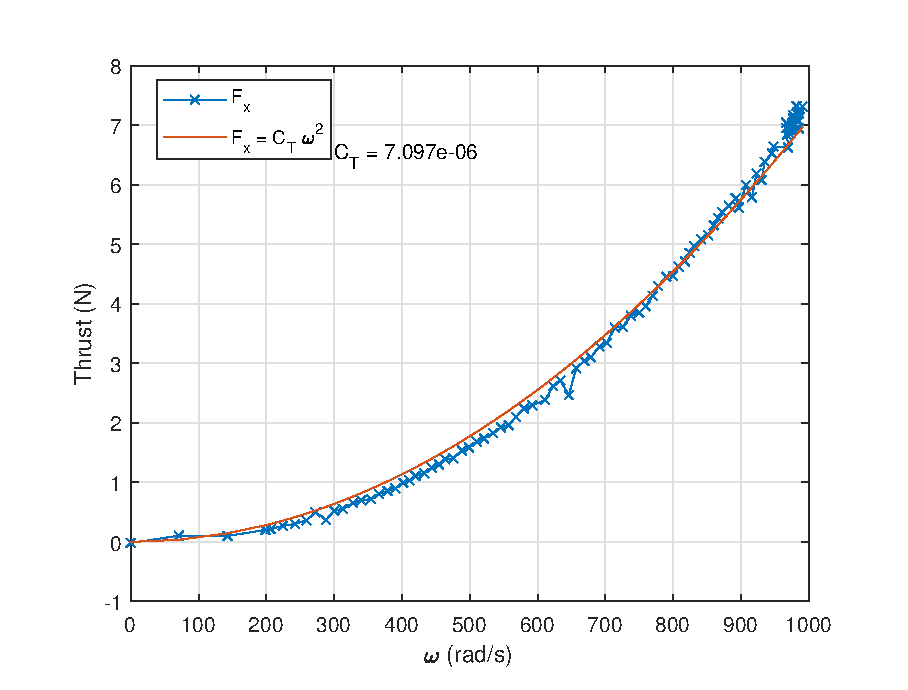
\includegraphics[width = \textwidth]{./figs/aero/Fx.eps}
        \end{figure}
        \caption{Variation of thrust with rpm}
    \end{minipage}
    \begin{minipage}{0.49\textwidth}
        \begin{figure}[H]
            \centering
            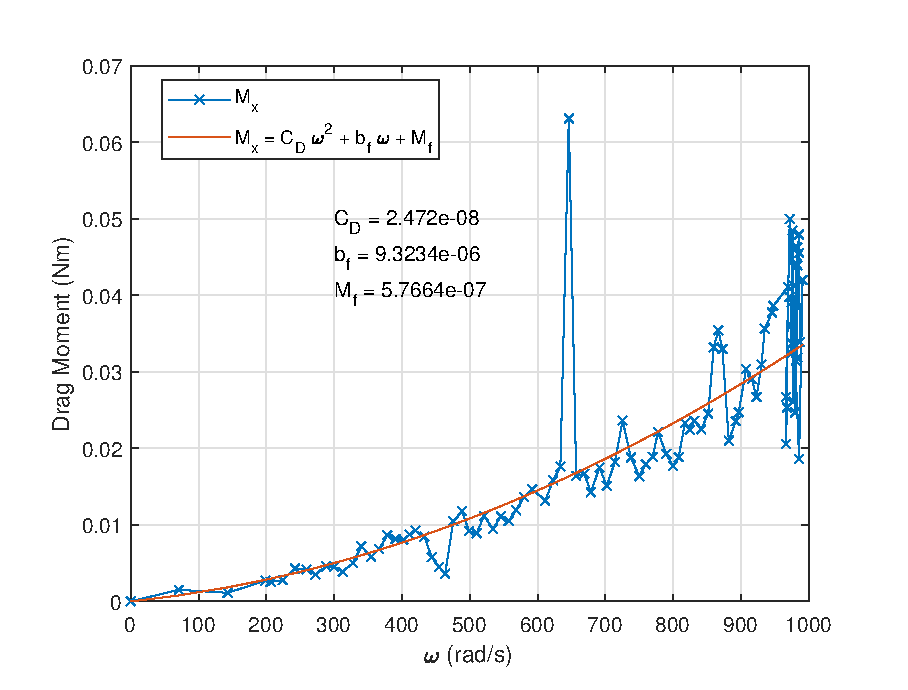
\includegraphics[width = \textwidth]{./figs/aero/Mx.eps}
            \caption{Variation of drag moment with rpm}
        \end{figure}
    \end{minipage}
\end{figure}

%===============================================================================
\newpage
\section{BLDC Motor Model}
\subsection{ESC and non-linear input compensation}

The torque and speed characteristics can be determined by the balance between motor's mechanical output power adn electrical input power over a conduction period:
\begin{align*}
    P &= \omega_m T_e = 2 e_p I\\
    e_p &= N_p B_g \pi r l \omega_m\\
    \text{Where, } \qquad &\\
    \omega_m &- \text{Mechanical rpm}\\
    T_e      &- \text{Electromagnetic torque}\\
    e_p      &- \text{Back emf}
\end{align*}

The factor 2 is the result of current flowing through 2-motor phases (trapesoidal wave form).\\

We have, electromagnetic torque:
\begin{align*}
    T_e &= 4 N_p B_g l r I &[\because \text{Lenz law}]
\end{align*}
let, $E = 2 e_p$. We have,
\begin{align*}
    E &= k \psi \omega_m = K_v \omega_m\\
    T_e &= k \psi I = K_T I\\
\text{Where, } \qquad &\\
    k &= 4 N_p  &(\text{Armature Constant})\\
    \psi &= B_g \pi  r l  &(\text{Flux})
\end{align*}

Thus, ideally back-emf constant and torque constants are same.\\

Using the above equations, the following steady-state torque speed characteristics can be drived. We have, the instantaneous voltage equation:
\begin{align*}
    V_s &= E + I R\\
\text{Where, } \qquad &\\
    V_s &- \text{Supply voltage}\\
    I &- \text{Total DC current}\\
    R &- \text{Sum of the terminal phase ressistances}
\end{align*}

We have torque speed relationship:
\begin{align*}
    \omega_m &= \omega_0 \left( 1 - \frac{T}{T_0} \right)\\
\text{Where, } \qquad &\\
    \omega_0 &= \frac{V_s}{k \psi} & (\text{No-load Speed})\\
    T_0 &= k \psi I_0              & (\text{Stall Torque})\\
    I_0 &= \frac{V_s}{R}           & (\text{Stall Current})
\end{align*}

\subsection{Dynamic Model (without Propeller)}
%===============================================================================
\newpage


\section{BLDC Motor with Propeller Model}
%===============================================================================
\newpage


\section{RPM sensing algorithm}
\subsection{Algorithm}
\subsection{Validation}
%===============================================================================
\newpage


\section{Static Model Parameter Identification}
\subsection{BLDC Motor}
\subsection{Propeller Aerodynamics}
%===============================================================================
\newpage


\section{Dynamic Model Parameter Identification}
\subsection{BLDC Motor}
\subsection{BLDC Motor and Propeller}
%===============================================================================
\newpage


\section{Conclusion: Model and Model Parameters}
\subsection{Parametric Form}
%===============================================================================
\newpage


\section{Gyroscopic Effects of Propeller Inertia}
%===============================================================================
\newpage
\newpage
\bibliographystyle{unsrt}
\bibliography{refs}

\end{document}
